\documentclass[10pt]{article}
\usepackage[dvips]{graphicx}
\usepackage{hyperref}
\usepackage{upquote}
\usepackage{wrapfig}
\usepackage{color}
\usepackage{colortbl}
\usepackage{hhline}
\usepackage{tabularx}
\oddsidemargin 0.25in
\evensidemargin 0.25in
\textwidth 6in
\textheight 8.5in
\topmargin -0.5in


\pagestyle{empty}
\begin{document}

\section*{Octave software note} Depending on your Octave installation, you may
need to install the signal processing package. That package defines the
\verb+dct+ fast discrete cosine transform function required by this project.
This is not required by MATLAB, which automatically loads the signal processing
functions by default.\\

Here is how you can set up Octave:

\begin{enumerate}
\item Start up Octave
\item Run the commands to install required packages (only required once):
\begin{verbatim}
pkg install -forge control
pkg install -forge signal
\end{verbatim}
\item Then before running this project (every time), run:
\begin{verbatim}
pkg load signal
\end{verbatim}
\end{enumerate}


\section*{Project 2: Digital Audio Compression}

The compression of digital audio data is an important topic.  Compressing
(reducing) the data storage requirements of digital audio allows us to fit more
songs into our phones and download them faster. We will apply ideas from
interpolation, least-squares and other topics to reduce the storage
requirements of digital audio files. All of our approaches will replace the
original audio signal with approximations that are made from a linear
combination of cosine functions.

You will learn the basic ideas behind data compression methods used in mp3 and
other algorithms. You'll also encounter several interesting MATLAB/Octave
commands in the course of this project, including commands for manipulating
sound.

\section*{Computers and sound}

Sound is a complicated phenomenon. It's normally caused by a moving object in
air (or other medium), for example a loudspeaker cone moving back and forth.
The motion in turn causes air pressure variations that travel through the air
like waves in a pond. Our eardrums convert the pressure variations into the
phenomenon that our brain processes as hearing.

Computers ``hear'' sounds using a microphone instead of an eardrum. The
microphone converts pressure variations into an electric potential with
amplitude corresponding to the intensity of the pressure. The computer then
processes the electrical signal using a technique called sampling. The computer
samples the signal by measuring its amplitude at regular intervals, often
44100 times per second. Each measurement is stored as a number with fixed
precision, often 16 bits. The following diagram illustrates the sampling
process showing a simple wave sampled at regular intervals\footnote{Image
adapted from Franz Ferdinand, \copyright 2005}:
\begin{center}
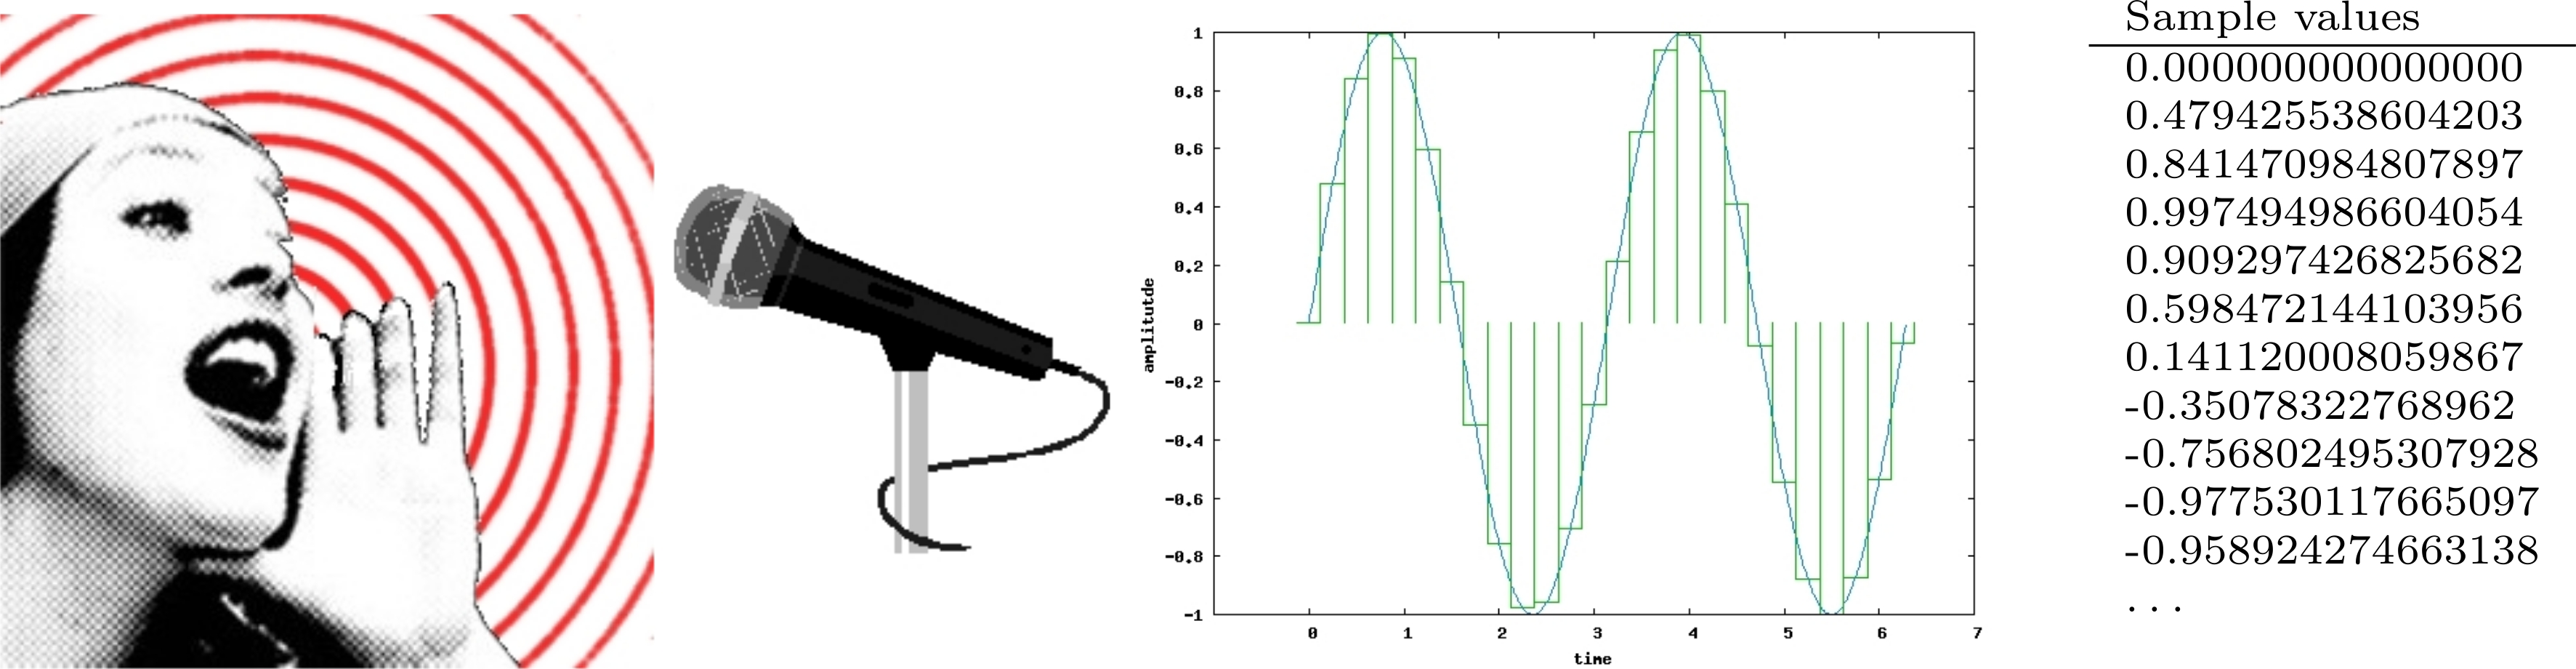
\includegraphics[width=5.5in]{fig1}
\end{center}

Computers emit sound by more or less reversing the above process. Samples are
fed to a device that generates an electric potential proportional to the sample
values. A speaker or other similar device then converts the electric signal
into air pressure waves.

The rate at which the measurements are made is called the {\it sampling rate}.
A common sampling rate is 44,100 times per second (used by compact disc, or CD,
audio). The numbers used to store the sampled audio signal are usually not
double-precision floating-point numbers (64 bits per number) but instead
lower-precision numbers. For example, compact discs use 16 bit numbers to store
their samples.

The {\it bit rate} of a set of digital audio data is the storage in bits
required for each second of sound. If the data has fixed sampling rate and
precision (like CD audio), the bit rate is simply their product. For example,
the bit rate of one channel of CD audio is 44100 samples/second $\times$ 16
bits/sample = 705600 bits/second. The bit rate is a general measure of
storage, and is not always simply the product of sampling rate and precision.
For example, we will presently encounter a way of encoding data with variable
precision.

    Large storage requirements limit the amount of audio that can be stored on
compact discs, flash memory and other media.  Large file sizes also work out to
long download times for retrieving songs from the internet. For these reasons
(and others), there is a lot of interest in shrinking the storage requirements
of sampled sound.


\section*{Least-squares data compression}

Least-squares data fitting can be thought of as a method for replacing a
(large) set of data with a model and a (smaller) set of model coefficients that
approximate the data in an 
\begin{wrapfigure}{r}{0.45\textwidth}
  \begin{center}
  \vspace{-20pt}
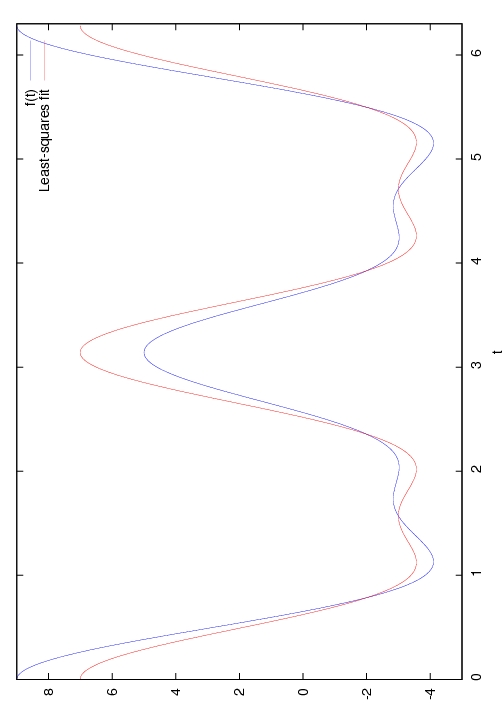
\includegraphics[angle=270,width=0.44\textwidth]{fig2}
  \end{center}
  \vspace{-50pt}
\end{wrapfigure}
optimal way--namely, by minimizing the
Euclidean norm of the residual difference between the data and the model.

Consider the following simple example. Let the function   
$f(t) = \cos(t) + 5\cos(2t) + \cos(3t) + 2\cos(4t).$ 
A plot of $f(t)$ for $0\le t\le 2\pi$ appears as the blue curve in the
figure. 
Let's say we are given a data set of 1000 discrete function values
of $f(t)$ regularly spaced over the interval $0\le t\le 2\pi$. We can fully
interpolate the data by setting up the model matrix A (using
MATLAB/Octave notation):
\begin{verbatim}
t = linspace (0,2*pi,1000)';
b = cos(t) + 5*cos(2*t) + cos(3*t) + 2*cos(4*t);
A = [ones(size(t)), cos(t), cos(2*t), cos(3*t), cos(4*t)];
\end{verbatim}
and then solving the linear system $Ax=b$ with the command 
{\verb@x=A\b@}. 
Try it! Note that the solution vector components match the function
coefficients.

Some of the coefficients are not as large as others in this simple example.
We can approximate the function $f$ with a least-squares approximation that
omits parts of the model corresponding to smaller coefficients.
For example, set up the least-squares model
\begin{verbatim}
A = [cos(2*t), cos(4*t)];
\end{verbatim}
and solve the corresponding least-squares system 
{\verb@x=A\b@}. 
This model uses only two coefficients to describe the data set of 1000
data points. The resulting fit is reasonable, and is displayed by the red
curve in the figure. The plot was made with the command
{\verb@plot (t,b,'-b',t,A*x,'-r')@}.

The cosine function oscillates with a regular frequency. The multiples of
$t$ in the above example correspond to different frequencies (the larger
the multiple of $t$ is, the higher the frequency of oscillation). 
The least-squares
fit computed the best approximation to the data using only two 
frequencies. 

\section*{Exercise}

{\bf Experiment with different least-squares models for the above example by
omitting different frequencies (that is--omitting different columns if
\verb@A@). Plot your experiments and briefly describe the results.}



\section*{Manipulating sound in MATLAB and Octave}

MATLAB and Octave provide lots of commands that make it relatively easy to read
in, manipulate, and listen to digital audio signals.  Accompanying this
project, you will find a short sound file:
\url{https://github.com/bwlewis/enr230-audio-compression/raw/main/shostakovich.wav}.
The file is sampled at 22050 samples per second and 16 bits per sample (exactly
1/2 the bit rate of CD audio), and is about 40 seconds long.  If you don't care
for the tune, you are free to experiment with any audio samples that you wish. 

The MATLAB/Octave command to load an audio file is:
\begin{verbatim}
%% download an audio file to 'tune.wav'...
urlwrite('https://github.com/bwlewis/enr230-audio-compression/raw/main/shostakovich.wav',...
         'shostakovich.wav');

%% read in the downloaded file...
[b,R] = audioread ('shostakovich.wav');
N = length(b);
\end{verbatim}
The returned vector b contains the sound samples (it's very long!), R is the
sampling rate, and N is the number of samples. Note that, even though the
precision of the data is 16 bits, MATLAB and Octave represent the samples as
double-precision internally. You can listen to the sample you just loaded with
the command:
\begin{verbatim}
sound (b,R);
\end{verbatim}

Some versions of MATLAB and Octave may have slightly different syntax--use the
help command for more detailed information. 
 
Sampled audio data is generally much more complicated looking than the simple
example in the last section, confirmed by viewing the data with the command
\verb@plot(b)@ (try it!). However, it too can be interpolated and/or
least-squares fit with a cosine model:
\[
y = c_0 + c_1\cos\omega_1t + c_2\cos\omega_2t + \cdots + c_{n-1}\omega_{n-1}t,
\]
for some positive integer $n-1$ and frequencies ${\omega_j}$.  A famous and
important result from information theory called the Shannon-Nyquist theorem
requires that the highest frequency in our model, $\omega_{n - 1}$,  be less
than half the sampling rate. That is, our cosine model assumes that the audio
data is filtered to cut-off all frequencies above half the sampling rate. 

The cosine model requires additional technical assumptions on the data.  Recall
that the cosine function is an even function, and the sum of even functions is
an even function. Therefore, the model also assumes that the data is even. The
usual approach taken to satisfy this requirement of the model is to simply
assume that the data is extended outside of the interval of interest to make it
even.

The above-mentioned conditions (cut-off frequency, extension beyond the
interval boundaries) are in general important to consider, but we won't get in
to the details in this project.  Instead, we focus on the basic ideas behind
compression methods like mp3. 

\subsection*{Computing the model interpolation coefficients with the DCT}

Let the vector $b$ contain one second of sampled audio, and assume that the
sampling rate is $N$ samples per second ($b$ is of length $N$).  It's tempting
to proceed just as in the simple example above by setting up an interpolation
model  (don't try this!):

\begin{verbatim}
t = linspace (0,2*pi,N)';
A = [ones(size(t)), cos(t), cos(2*t), cos(3*t), ..., cos((N/2-1)*t)];
x = A\b;
\end{verbatim}
Aside from a few technical details, this method could be used to interpolate
an audio signal. However, consider the size of the quantities involved.
At the CD-quality sampling rate, $N=44100$, and the matrix $A$ is
gigantic ($44100\times 22050$)!  This problem is unreasonably large.


Fortunately, there exists a remarkable algorithm called the Fast Discrete
Cosine Transform (DCT) that can compute the solution with extreme efficiency.
The DCT is a variation on the famous fast Fourier transform (FFT)--one of the
most important algorithms ever devised. The DCT produces scaled versions of the
model coefficients for us with the command:
\begin{verbatim}
c = dct(b);
\end{verbatim}
The returned coefficient vector $c$ is of the same length as $b$. 

To investigate the plausibility of the DCT, we can try it out on our
simple example:
\begin{verbatim}
% Simple example revisited
t = linspace (0,2*pi,1000)';
b = cos(t) + 5*cos(2*t) + cos(3*t) + 2*cos(4*t);
x = dct(b);
N = length(b);
w = sqrt(2/N);
f = linspace(0, N/2, N)';
plot (f(1:8),w*x(1:8),'x');
\end{verbatim}
The variable $w$ is a scaling factor produced by the DCT algorithm and
the vector $f$ is the frequency scale for the model coefficients 
computed by the DCT and stored in $x$.
The frequency range from $0$ to $N/2 - 1$ corresponds to half
the sampling rate (assumed here to be $N$).
We can think of the \verb@dct(b)@ command as essentially computing
\verb@A\b@ for the full interpolation model using the frequencies
in the vector $f$.
Your plot should show that we closely compute the model coefficients 
(i.e., a value of $1$ at frequency $1$, $5$ at frequency $2$, etc.)

We can reconstruct the original signal from the model coefficients with
the command:
\begin{verbatim}
y = idct(x);     % The reconstructed data is in y.
plot (t, b, '-r', t, y,'-b');
\end{verbatim}
The plots should overlay each other. The \verb@idct@ command is the inverse
of the {\tt dct} command. We can think of {\tt idct(x)} as 
computing the product $Ax$ for an appropriate model matrix $A$ and
coefficient vector $x$.




\section*{Digital filtering}

The DCT algorithm can be used to not only interpolate data, but to compute a
least-squares fit to the data by omitting frequencies.  The process of
computing a least-squares fit to digitized signals by omitting frequencies is
called digital filtering.  Digital filtering can reduce the storage
requirements of digital audio by simply lopping off parts of the data that
correspond to specific frequencies.  Of course, cutting out frequencies affects
the sound quality of data.  However, the human ear is not equally sensitive to
all frequencies.  In particular, we generally don't perceive very high and very
low frequencies nearly as well as mid-range frequencies.  In some cases, we can
filter out these frequencies without significantly affecting quality.  An easy
way to filter specific frequencies in MATLAB and Octave is to generate a mask.
Consider this example:

\begin{verbatim}
[b,R] = audioread('shostakovich.wav');
N = length(b);
c = dct(b);                % Compute the interpolation model coefficients
w = sqrt(2/N);
f = linspace(0, R/2, N)';
plot (f,w*c);     % Shows a plot of the frequencies coefficients for the sample
% Generate a mask of zeros and ones. m is 0 for every frequency above 2000, 1 otherwise.
% This mask will cut-off all frequencies above 2000 cycles/second.
m = (f < 2000);
plot (f, w*m .* c);   % Display the filtered frequency coefficients.
y = idct(m .* c);     % Generate a filtered sound sample data set
sound(y, R);          % Listen to the result!
\end{verbatim}

\section*{Exercise}
{\bf Experiment with several frequency cut-off values in the above example.
Listen to your results. }

\section*{Exercise}
{\bf Exhibit how to construct a single mask that will
cut off frequencies below 200 {\it and} above 5000 cycles/second. }

\section*{Exercise}
{\bf How much does the above code reduce the storage requirement of the sample
(in bit rate)?}

\section*{The ideas behind mp3}
Digital fifiltering is an effective technique for compressing audio
data in many situations, especially telephony. Cutting out entire
frequency ranges is rather a brute-force method, however. There are
more effective ways to reduce the storage required of digital audio
data, while also maintaining a high-quality sound.

One idea is this: rather than cutting out ``less-important'' 
frequencies altogether, we could store the corresponding model 
coefficients with lower precision--that is, with fewer bits. 
This technique is called quantization.

\begin{wrapfigure}{r}{0.45\textwidth}
  \begin{center}
  \vspace{-30pt}
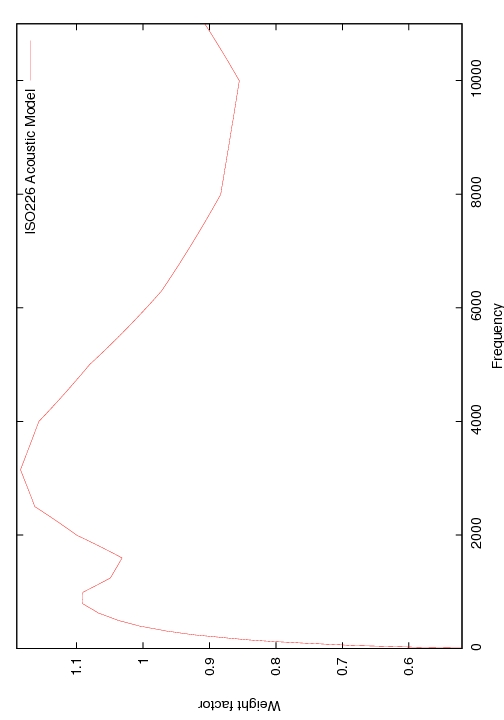
\includegraphics[angle=270,width=0.44\textwidth]{fig3}
  \end{center}
  \vspace{-20pt}
\end{wrapfigure}
We've already encountered that we don't hear all frequencies
equally well. This phenomenon has been studied extensively, and as
a result we have a pretty good model of ``average'' human frequency
perception. 
The fifigure shows an example perceptual
frequency response curve from zero to 11kHz 
adapted from an international standard ISO226, 
generated with the psyweight and iso226 functions included with this project. 
We can use such models to help determine which frequencies
in a data set are important, and which ones are less important to the 
perceived sound.
We will then store the less-important frequencies with less precision.
The idea is to focus the compression on parts of the signal that are
perceptually less important.

Here is an illustration of an audio compression method similar to
(but much simpler than) mp3 compression:
\begin{figure}[h!]
\begin{center}
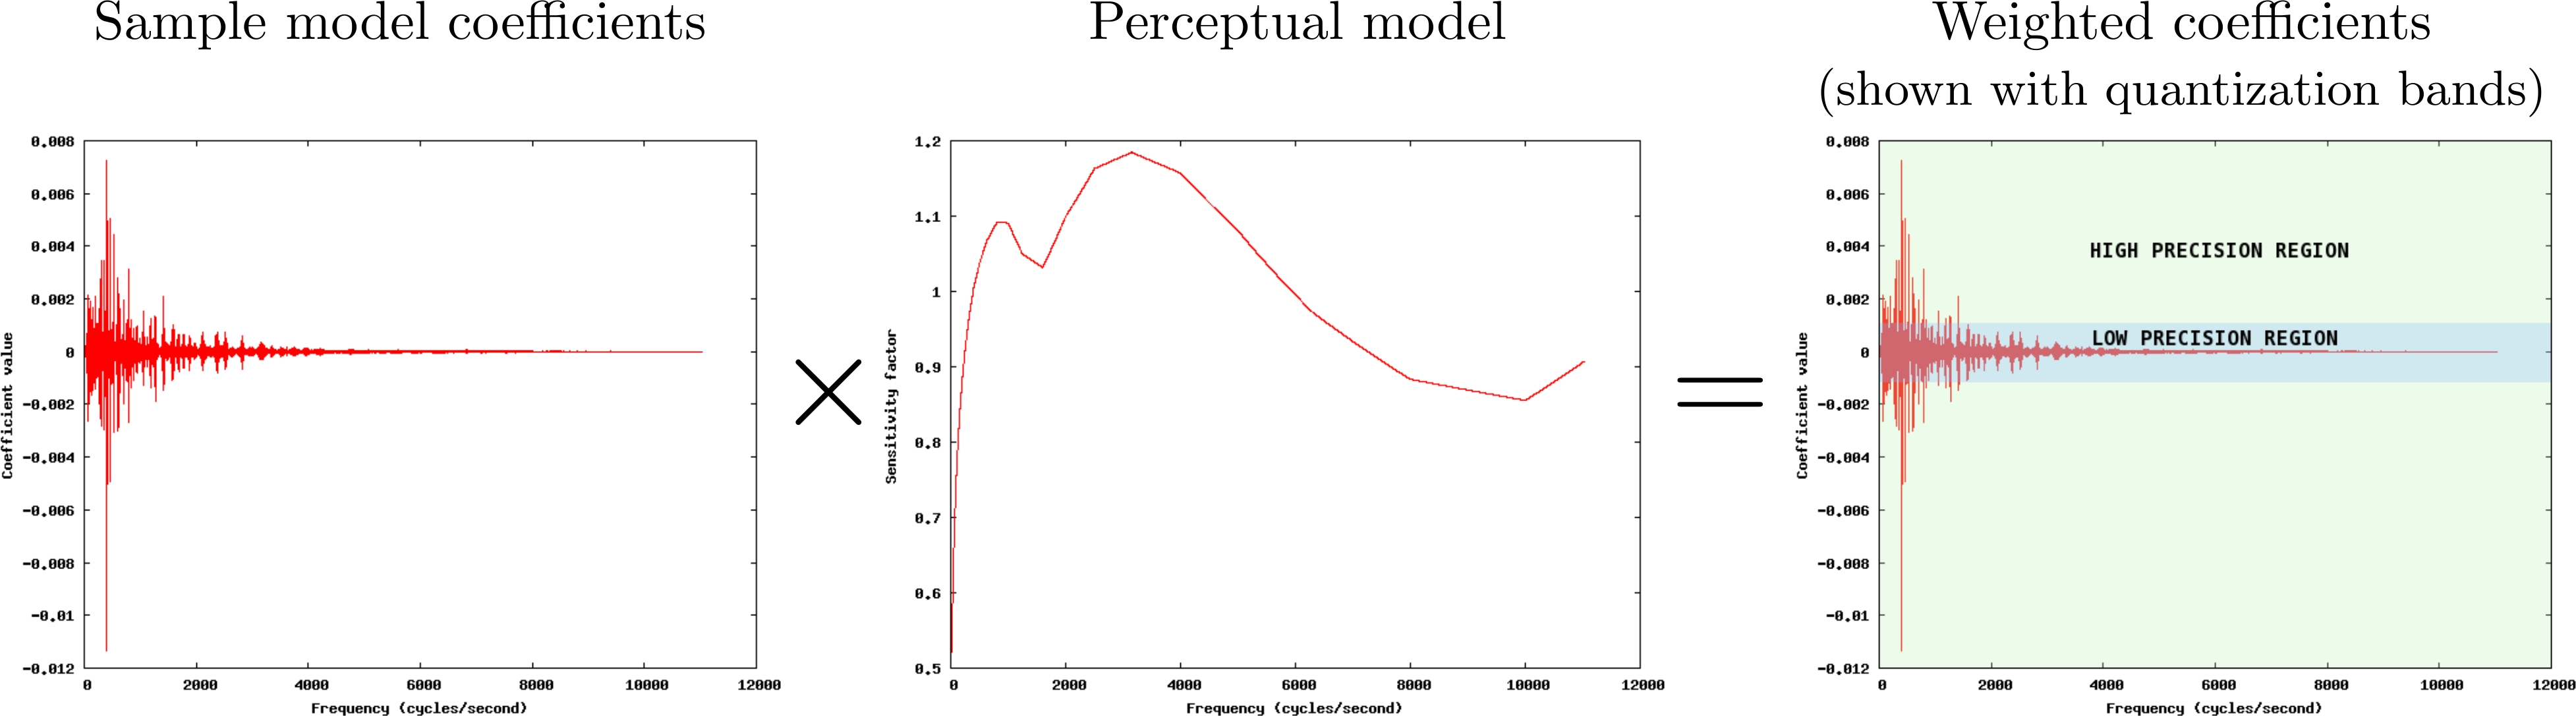
\includegraphics[width=0.98\textwidth]{fig4}
\end{center}
\end{figure}
Note that with the illustrated choice of quantization bands, the bulk of
the model coefficients lie in the low precision storage realm in the 
above example. Our compression method will encode all of the corresponding
unweighted model coefficients that fall in that band with low precision.
Note that the perceptual model is only used to help decide which coefficients
are important to keep at full precision. The precise cutoff between low-
and high-precision storage will govern the overall compression obtained
by this method.

For example, let's say that 90\% of the coefficients lie in the 
low-precision part of the illustration. Suppose that we store those
coefficients with only 8-bit numbers, and the remaining ones with
16-bit numbers. The resulting data will only require about 55\% of the
storage space used by the original sample data set of entirely 16-bit
numbers.
\section*{Exercise}
{\bf What is the bit rate of the compressed audio sample discussed in the
last paragraph, assuming 22,050 samples per second?}
\\[8pt]
We can achieve higher compression by either widening the low-precision
region, or by lowering the precision used to store the coefficients, or
both. The algorithm used in mp3 compression uses similar techniques to
achieve up to a 10:1 compression of CD audio and still maintain a high
perceived quality of sound.

\subsection*{Quantization in MATLAB and Octave}

MATLAB and Octave do not easily represent quantized numbers internally. 
We can, however, simulate the result of quantization in double-precision
with the following function, {\tt quantize.m}:
\begin{verbatim}
function y = quantize (x, bits)

m = max(abs(x));
y = x/m;
y = floor((2^bits - 1)*y/2);
y = 2*y/(2^bits -1);
y = m*y;

\end{verbatim}
%%\section*{Exercise}
%%{\bf Explain how the quantize.m function works.}



\section*{MP3-like compression with MATLAB and Octave}

Before proceeding you will need to download the functions \verb+psyweight.m+
and \verb+iso226.m+:

\begin{verbatim}
baseurl = 'https://raw.githubusercontent.com/bwlewis/enr230-audio-compression/main/';
urlwrite([baseurl, 'quantize.m'], 'quantize.m');
urlwrite([baseurl, 'iso226.m'], 'iso226.m');
urlwrite([baseurl, 'psyweight.m'], 'psyweight.m');
\end{verbatim}


The following code example illustrates our discussion of audio data compression
with actual audio samples. You will need the above {\tt quantize.m} function,
as well as the standard perceptual model of human hearing provided in the
functions {\tt psyweight.m} and {\tt iso226.m}. 
\begin{verbatim}
[b,R] = audioread ('shostakovich.wav');    % Load an audio sample
N  = length(b);
c = dct(b);        % Compute the interpolation model coefficients
w = sqrt(2/N);
f = linspace(0,R/2,N)';
% Generate a perceptual model (requires psyweight.m, iso226.m)
p = psyweight(f);
% Let’s look at the weighted coefficients and pick a cutoff value
plot (f,w*p.*c)

% Pick a cutoff value and split the coefficients into low- and high-precision sets:
cutoff = 0.00015
mask = (abs(w*c)<cutoff);
low = mask .* c;
high = (1-mask) .* c;
% This plot illustrates the cutoff region:
plot(f,w*high,'-r',f,w*low,'-b')

% Now pick a precision (in bits) for the low precision data set:
lowbits = 8
% We won’t quantize the high-precision set of coefficients (high), only the
% low precision part (requires quantize.m): 
low = quantize(low, lowbits);

% Finally, let's reconstruct our compressed audio sample and listen to it!
y = idct(low+high);
sound (y,R);
\end{verbatim}
\section*{Exercise}
{\bf Experiment with the above code, trying out different cutoff values (\verb+cutoff+)
and precision values (\verb+lowbits+). Listen to your results. What is the 
lowest bit rate that you can find that still sounds good to you?}

\end{document}
